\clearpage

\section{A SICStus \clpq és \clpr könyvtárai}

A következõ fejezetben a SICStus \clpq, illetve \clpr könyvtáraival
fogunk foglalkozni.

\subsection{A \clpq és \clpr könyvtár általános jellemzése}

A \clpq könyvtár egy, a racionális számok tartományára
alapuló CLP rendszert valósít meg, a \clpr könyvtár pedig ugyanezt, csak
lebegõpontos formában ábrázolt valós számokkal. A felhasználható függvények
tartalmazzák az alapmûveleteket (\cd{+ - * /}), valamint több magasabb rendû
mûveletet is (\cd{min}, \cd{max}, \cd{exp}, \cd{abs}, \cd{sin}, \cd{tan}\ldots).
Korlát-relációnak a valós számok között fennálló alapvetõ relációkat
használhatjuk (\cd{= =:= < > =< >= =\bs=}). Egyszerû korlátoknak a lineáris
összefüggéseket tartalmazó korlátokat tekintjük, a korlátmegoldó algoritmus
a Gauss-elimináción és a szimplex módszeren alapul. A könyvtárakat az alábbi
parancsokkal vehetjük használatba:

\begin{verbatim}
:- use_module(library(clpq)).
:- use_module(library(clpr)).
\end{verbatim}

A korlát-tárat a CLP(MiniNat)-hoz hasonlóan a \cd{\{Korlát\}} alakú
kifejezésekkel bõvíthetjük, ahol \cd{Korlát} egy változókból és egész vagy
lebegõpontos számokból a fenti mûveletekkel felépített reláció, vagy
ilyen relációk vesszõvel elválasztott konjunkciója.
\br
Mivel a \clpq és a \clpr könyvtárak nagy mértékben hasonlítanak
egymásra, ezért a továbbiakban csak a \Clpq-val foglalkozunk, de az
elmondottak ugyanúgy érvényesek a \Clpr-re is.

\subsection{Egy példafutás a \clpq könyvtár segítségével}

Az alábbiakban egy rövid példán keresztül fogjuk bemutatni a \clpq
könyvtár használatát.
\br
Elõször be kell töltenünk a \clpq könyvtárat, hogy használatba vehessük:

\begin{verbatim}
| ?- use_module(library(clpq)).
{ loading ../library/clpq.ql.. }
.. .. ..
\end{verbatim}

Egyszerû korlátok felvétele (lineáris egyenletrendszer megoldása):

\begin{verbatim}
| ?- {X=Y+4, Y=Z-1, Z=2*X-9}.   
X = 6, Y = 2, Z = 3 ?
\end{verbatim}

Ha a beadott korlátoknak még nincs egyértelmû megoldása, akkor a
\clpq rendszer a fennálló relációkat (a korlát-tár állapotát)
írja ki, mint például az alábbi lineáris egyenlõtlenségnél:

\begin{verbatim}
| ?- {X+Y+9<4*Z, 2*X=Y+2, 2*X+4*Z=36}.  
{X<29/5}, {Y= -2+2*X}, {Z=9-1/2*X} ?    
\end{verbatim}

Mint már említettük, a \clpq rendszer csak lineáris korlátokat
tud felvenni a korlát-tárba, elõfordulhat azonban, hogy egy nemlineáris
korlátot linearizálni tud. Ilyen esetben a nemlineáris korlát lineáris
megfelelõje be tud kerülni a korlát-tárba. Az alábbi példa egy olyan esetet
mutat, amikor egy kifejezés két különbözõ, de ekvivalens alakját beadva az
egyik a linearizálás miatt be tud kerülni a korlát-tárba, míg a másik nem:

\begin{verbatim}
| ?- {(Y+X)*(X+Y)/X = Y*Y/X+100}.       
{X=100-2*Y} ?            % lineárissá válik

| ?- {(Y+X)*(X+Y) = Y*Y+100*X}.         
                         % így már nem lineáris
clpq:{2*(X*Y)-100*X+X^2=0} ?             
                         % a clpq modul-prefix jelzi,
                         % hogy felfüggesztett összetett
                         % hívásról van szó
\end{verbatim}

Tisztán nemlineáris korlátok minden esetben a táron kívül maradnak, persze
elõfordulhat, hogy a nemlineáris korlát egy késõbbi egyesítés vagy
változóbehelyettesítés miatt lineárissá válik, mint ahogy az alábbi
példa is mutatja:

\begin{verbatim}
| ?- {exp(X+Y+1,2) = 3*X*X+Y*Y}.        
                         % nem lineáris...
clpq:{1+2*X+2*(Y*X)-2*X^2+2*Y=0} ? 

| ?- {exp(X+Y+1,2) = 3*X*X+Y*Y}, X=Y.   
X = -1/4, Y = -1/4 ?     % így már igen...
\end{verbatim}

Persze a nemlineáris korlátok is megoldhatóak:

\begin{verbatim}
| ?- {2 = exp(8, X)}.
X = 1/3 ?
\end{verbatim}

\subsection{Összetett korlátok kezelése \Clpq-ban}

Ahogy azt már említettük, \Clpq-ban és \Clpr-ben összetett korlátnak
számítanak a nemlineáris (vagy a rendszer által nem linearizálható, de
egyébként lineáris) kifejezések, ezek nem kerülnek be a korlát-tárba, hanem
démonként várakoznak arra, hogy lineárissá válva bekerülhessenek oda.
Fontos megjegyezni, hogy a \Clpq-ban és a \Clpr-ben a démonok
\emph{semmiféle} erõsítõ tevékenységet nem végeznek, kizárólag akkor
módosíthatják a tárat, ha valamilyen behelyettesítés folyamán lineárissá
válnak. Ez gyengébb az általános korláterõsítõ mechanizmusnál. Ennek
bizonyítására képzeljük el a következõ példát: a korlát-tár tartalma legyen
az \cd{X > 3} korlát, a nemlineáris korlát pedig az \cd{Y > X*X}. A
korlátmegoldó ennek alapján kikövetkeztethetné, hogy \cd{Y > 9}, és ezt
fel is vehetné a korlát-tárba, hiszen ez már lineáris korlát (persze emellett
az \cd{Y > X*X} démont továbbra is életben kell hagynia). A \cd{clpq/r} ezt
nem teszi meg, és így nyilvánvalóan nem használja fel ezt az információt
a további következtetésekhez.
\br
Lássunk egy további példát az összetett korlátokra vonatkozóan!

\begin{verbatim}
| ?- {X =< Y}, {X*(Y+1) > X*X+Z}, 
       (   Z = X*(Y-X), {Y < 0}
       ;   Y = X
       ).
                        Y = X,  {X-Z>0} ? ; no
\end{verbatim}

Nézzük meg, hogyan jött ki a fenti eredmény! A rendszer a fenti célsorozat
futtatásakor választási pont létrehozása nélkül felveszi az elsõ két korlátot
a korlát-tárba, ezt az alábbi célsorozat futtatásával ellenõrizhetjük:

\begin{verbatim}
| ?- {X =< Y}, {X*(Y+1) > X*X+Z}.
                        {X-Y=<0}, clpq:{Z-X-Y*X+X^2<0} ?
\end{verbatim}

A sor végén jól látható a várakozó démon is. Ezek után egy választási pont
következik, és az elsõ ágon továbbhaladva felvesszük a \cd{Z}-re vonatkozó
korlátot:

\begin{verbatim}
| ?- {X =< Y}, {X*(Y+1) > X*X+Z}, Z = X*(Y-X).
                        Z = X*(Y-X), {X-Y=<0}, {X>0} ? 
\end{verbatim}

Látható, hogy a démonunk felébredt, és egyszerû korláttá válva bekerült a
korlát-tárba. Ha ezek után megérkezik az \cd{Y}-ra vonatkozó korlát, akkor
ez ellentmondásban lesz a korlát-tár eddigi tartalmával, hiszen ha \cd{X}
pozitív (lásd az elõzõ futás eredményében az utolsó korlátot), és \cd{Y}
negatív, akkor \cd{X-Y} mindenképp pozitív, ami ellentmondásban van azzal
a korláttal, hogy \cd{X-Y=<0}. Ezt a rendszer egy meghiúsulás formájában
,,éli át'':

\begin{verbatim}
| ?- {X =< Y}, {X*(Y+1) > X*X+Z}, Z = X*(Y-X), {Y < 0}.
                        no
\end{verbatim}

A meghiúsulás miatt a korlát-tár tartalma visszafejtõdik egészen a választási
pontnál fennálló helyzetig, ahonnan a másik ágon fut tovább, és ott meg is
találjuk az egyetlen megoldást:

\begin{verbatim}
| ?- {X =< Y}, {X*(Y+1) > X*X+Z}, Y = X.
                        Y = X, {X-Z>0} ? 
\end{verbatim}

\subsection{Bonyolultabb \clpq példa: hiteltörlesztés}

\begin{verbatim}
% Hiteltörlesztés számítása: P összegû hitelt
% Time hónapon át évi IntRate kamat mellett havi MP
% részletekben törlesztve Bal a maradványösszeg.
mortgage(P, Time, IntRate, Bal, MP):-
     {Time > 0, Time =< 1,
     Bal = P*(1+Time*IntRate/1200)-Time*MP}.
mortgage(P, Time, IntRate, Bal, MP):-
     {Time > 1},
     mortgage(P*(1+IntRate/1200)-MP, 
              Time-1, IntRate, Bal, MP).
\end{verbatim}

A fenti \clpq példa további magyarázatot nem igényel, érdemes azonban
megfigyelnünk, hogy a \clpq természetébõl adódóan az eljárás hívásakor
nem kötelezõ úgy kitöltenünk a paramétereket, hogy azokból egyértelmûen
következzen a megoldás, ugyanis ha ez nem teljesül, akkor a \clpq
kifejezi a hiányzó adatokat a megadottak függvényében:

\begin{verbatim}
| ?- mortgage(100000,180,12,0,MP).
                        % 100000 Ft hitelt 180        
                        % hónap alatt törleszt 12%-os 
                        % kamatra, mi a havi részlet?                 
MP = 1200.1681 ? 

| ?- mortgage(P,180,12,0,1200).         
                        % ugyanez visszafelé
P = 99985.9968 ? 

| ?- mortgage(100000,Time,12,0,1300).   
                        % 1300 Ft-ot törleszt havonta,
                        % hány hónapig kell törleszteni?                      
Time = 147.3645 ? 

| ?- mortgage(P,180,12,Bal,MP). 
{MP=0.0120*P-0.0020*Bal} ? 

| ?- mortgage(P,180,12,Bal,MP), ordering([P,Bal,MP]).
{P=0.1668*Bal+83.3217*MP} ? 
\end{verbatim}

Az \cd{ordering/1} predikátum egy listát vár paraméterként, és ezzel a
listával megadhatjuk, hogy az eredményben milyen sorrendben szerepeljenek
a változók. Ezzel gyakorlatilag azt is szabályozhatjuk, hogy melyik változót
melyikek segítségével fejezze ki a rendszer. A fenti példában \cd{P} áll a
lista elsõ helyén, ezért \cd{P}-t fogja kifejezni a többi segítségével.

\subsection{További könyvtári eljárások}

\begin{itemize}
\item \cd{entailed(Korlát)} --- sikerül, ha \cd{Korlát} levezethetõ a
jelenlegi tárból, meghiúsul, ha nem

\item \cd{inf(Kif,Inf), sup(Kif,Sup)} --- kiszámolja \cd{Kif} infimumát,
illetve szuprémumát, és egyesíti \cd{Inf}-fel, illetve \cd{Sup}-pal.
Példa:

\begin{verbatim}
| ?- { 2*X+Y =< 16, X+2*Y =< 11, X+3*Y =< 15, Z = 30*X+50*Y }, sup(Z, Sup).
Sup = 310, {....}
\end{verbatim}

\item \cd{minimize(Kif), maximize(Kif)} --- kiszámolja \cd{Kif} infimumát,
illetve szuprémumát, és egyesíti \cd{Kif}-fel. Példa:

\begin{verbatim}
| ?- { 2*X+Y =< 16, X+2*Y =< 11, X+3*Y =< 15, Z = 30*X+50*Y }, maximize(Z).
X = 7, Y = 2, Z = 310 ?
\end{verbatim}

\item \cd{bb_inf(Egészek, Kif, Inf)} --- kiszámolja \cd{Kif} infimumát,
azzal a további feltétellel, hogy az \cd{Egészek} listában levõ minden
változó egész (ún. ,,Mixed Integer Optimisation Problem'').

\begin{verbatim}
| ?- {X >= 0.5, Y >= 0.5}, inf(X+Y, I).
I = 1, {Y>=1/2}, {X>=1/2} ?

| ?- {X >= 0.5, Y >= 0.5}, bb_inf([X,Y], X+Y, I).
I = 2, {X>=1/2}, {Y>=1/2} ?
\end{verbatim}

\item \cd{ordering(V1 < V2)} --- A \cd{V1} változó elõbb szerepeljen az
eredmény-korlátban mint a \cd{V2} változó.

\item \cd{ordering([V1,V2,...])} --- \cd{V1, V2, ...} ebben a sorrendben
szerepeljen az eredmény-korlátban.

\end{itemize}

\subsection{A \clpq és a \clpr belsõ számábrázolása}

A \clpr lebegõpontos szám formátumban tárolja a számokat, itt tehát
semmi különlegességgel nem találkozhatunk. A \clpq azonban racionális
számokkal dolgozik, és ezeket a számokat egy \cd{rat(Számláló,Nevezõ)}
alakú struktúrával ábrázolja, ahol a tört számlálója és nevezõje mindig
relatív prím. Ennek bizonyítására tekintsük az alábbi \clpq példákat:

\begin{verbatim}
| ?- {X=0.5}, X=0.5.
no
| ?- {X=0.5}, X=1/2.
no
| ?- {X=0.5}, X=rat(2,4).
no
| ?- {X=0.5}, X=rat(1,2).
X = 1/2 ?
| ?- {X=5}, X=5.
no
| ?- {X=5}, X=rat(5,1).
X = 5 ?
\end{verbatim}

\subsection{Egy nagyobb \clpq feladat: tökéletes téglalapok}

\label{teglalap:clpqr}

A feladat: egy olyan téglalap keresése, amely kirakható páronként különbözõ
oldalú négyzetekbõl.

\enumhead{Egy lehetséges megoldás}
(a legkevesebb, 9 db négyzet felhasználásával)
\begin{center}
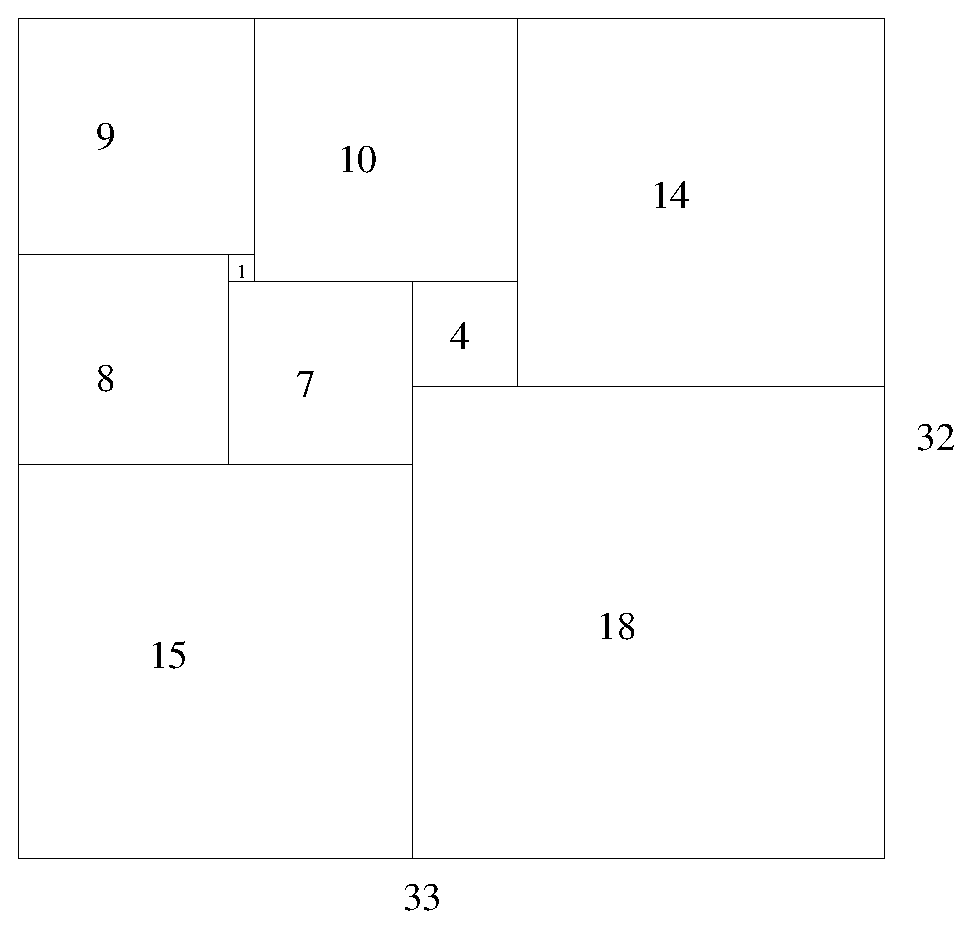
\epsfig{file=tokeletes.eps,width=0.4\textwidth}
\end{center}

A feladat megoldása során a négyzetet a ,,tetris-elv'' alapján, alulról
felfelé és balról jobbra fogjuk kitölteni, tehát a következõ négyzetet
mindig igyekszünk a négyzetben lent és bal oldalt elhelyezni, ameddig
ez lehetséges. Mivel a fenti elv alapján töltjük ki a négyzetet, ezért a
ki nem töltött terület összefüggõ, ezért jellemezhetõ a körvonalával, amit
Prologban egy listával fogunk lekódolni, amelyben a vonal függõleges és
vízszintes szakaszainak hosszát adjuk meg egy adott körüljárási sorrend
szerint. A függõleges és vízszintes szakaszok váltakozva fordulnak elõ,
ezért a listánkban minden páratlanadik elem függõleges szakaszt, minden
párosadik elem vízszintes szakaszt fog kódolni. A körüljárást a négyzet
bal felsõ sarkából kezdjük az óramutató járásával ellenkezõ irányban, és
a lista utolsó elemét elhagyjuk, mivel a körvonal záródása miatt ez úgyis
redundáns. Ezek alapján például egy 33 $\times$ 32-es üres négyzet a
\cd{[-32,33,32]} listával kódolható. Ha tekintjük a fenti négyzetet abban
az állapotban, amikor csak a 15 oldalhosszúságú négyzetet helyeztük el,
akkor az üres területet a \cd{[-17,15,-15,18,32]} lista írja le.
\br
A keresési terünkben kétfajta választási pont fog elõfordulni: vízszintes
és függõleges. Függõleges választási pontnál azt döntjük el, hogy amikor
egy négyzet mellé egy másik négyzetet lerakunk, akkor az új négyzet magassága
milyen relációban álljon a már lerakott négyzettel. Vízszintes választási
pontnál azt döntjük el, hogy a már kiválasztott oldalhosszúságú négyzet
mellett mekkora üres helyet hagyjunk még a kitöltésben. Ezt a két választási
pontot szemlélteti az alábbi ábra:

\begin{center}
\begin{tabular}{cc}
Vízszintes választási pont & Függõleges választási pont
\\
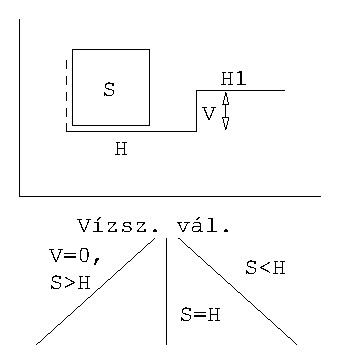
\epsfig{file=rect_choice_v.eps,width=0.4\textwidth}
&
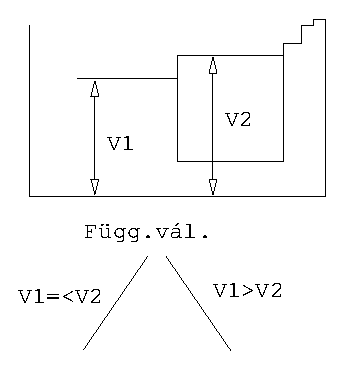
\epsfig{file=rect_choice_f.eps,width=0.4\textwidth}
\end{tabular}
\end{center}

A fentiekhez még annyi kiegészítés szükséges, hogy a programban a
négyzet függõleges oldalát mindig 1-nek választjuk, így csak a vízszintes
oldal méretével kell variálni. A megoldáshoz használt predikátumok:

\begin{verbatim}
% Colmerauer A.: An Introduction to Prolog III, 
% Communications of the ACM, 33(7), 69-90, 1990. 
\end{verbatim}
\begin{verbatim}
% Rectangle 1 x Width is covered by distinct 
% squares with sizes Ss.
filled_rectangle(Width, Ss) :-
       { Width >= 1 }, distinct_squares(Ss),
       filled_hole([-1,Width,1], _, Ss, []).
\end{verbatim}
\begin{verbatim}
% distinct_squares(Ss): All elements of Ss are distinct.
distinct_squares([]).
distinct_squares([S|Ss]) :-
       { S > 0 }, outof(Ss, S), distinct_squares(Ss).
\end{verbatim}
\begin{verbatim}
outof([],     _).
outof([S|Ss], S0) :- { S =\= S0 }, outof(Ss, S0).
\end{verbatim}
\begin{verbatim}
% filled_hole(L0, L, Ss0, Ss): Hole in line L0
% filled with squares Ss0-Ss (diff list) gives line L.
% Def: h(L): sum of lengths of vertical segments in L.
% Pre: All elements of L0 except the first >= 0.
% Post: All elems in L >=0, h(L0) = h(L).
filled_hole(L, L, Ss, Ss) :-
       L = [V|_], {V >= 0}.
filled_hole([V|HL], L, [S|Ss0], Ss) :-
       { V < 0 }, placed_square(S, HL, L1),
       filled_hole(L1, L2, Ss0, Ss1), { V1=V+S },
       filled_hole([V1,S|L2], L, Ss1, Ss).
\end{verbatim}
\begin{verbatim}
% placed_square(S, HL, L): placing a square size S on
% horizontal line HL gives (vertical) line L.
% Pre: all elems in HL >=0
% Post: all in L except first >=0, h(L) = h(HL)-S.
placed_square(S, [H,V,H1|L], L1) :- 
       { S > H, V=0, H2=H+H1 }, 
       placed_square(S, [H2|L], L1).
placed_square(S, [S,V|L], [X|L]) :- { X=V-S }.
placed_square(S, [H|L], [X,Y|L]) :- 
       { S < H, X= -S, Y=H-S }.
\end{verbatim}

A program belépési pontja a \cd{filled_rectangle/2} predikátum, amely
a \cd{Width} paraméterében fogja megadni a téglalap szélességét, \cd{Ss}-ben
pedig a kitöltéshez felhasznált négyzetek listáját. A \cd{distinct_squares/1}
korlát adja meg, hogy a négyzeteknek nem lehetnek azonos méretûek. Ez egy
egyszerû ,,darálás'' az \cd{Ss} listában elõforduló összes négyzet-párra
az \cd{outof/2} segítségével. A négyzetek elhelyezését a \cd{filled_hole/4}
predikátum végzi. A predikátum harmadik és negyedik paramétere a kezdõ-
és a végállapotban elhelyezett négyzetek listáját adja, az elsõ és a második
paraméter pedig a harmadik és negyedik paraméterben leírt állapothoz tartozó
határoló vonalak leírása a fentebb leírt formában. A \cd{placed_square/3}
predikátum pedig a vízszintes választási pontok három fajtáját írja le,
mégpedig azt, hogy ilyen esetben a határoló vonal milyen szabályok szerint
változik.
\br
Lássunk egy példafuttatást:
\begin{verbatim}
% 600 MHz Pentium III
| ?-    length(Ss, N), N > 1, statistics(runtime, _),
        filled_rectangle(Width, Ss), 
        statistics(runtime, [_,MSec]).

N = 9, MSec = 8010, Width = 33/32,
Ss = [15/32,9/16,1/4,7/32,1/8,7/16,1/32,5/16,9/32] ? ;

N = 9, MSec = 1010, Width = 69/61,
Ss = [33/61,36/61,28/61,5/61,2/61,9/61,25/61,7/61,16/61] ? ;

N = 9, MSec = 10930, Width = 33/32,
Ss = [9/16,15/32,7/32,1/4,7/16,1/8,5/16,1/32,9/32] ? 
\end{verbatim}
Amint látható, 9-nél kevesebb négyzettel nem lehet lefedni a téglalapot,
9-re viszont máris három megoldást talált a program, ebbõl az elsõ és
a harmadik csak a négyzetek elhelyezésében különbözik.
\br
A program mûködésének megértéséhez hagyjuk ki az \cd{outof/2} által
generált korlátokat, és nézzük meg, hogy kisebb méretû téglalapokra milyen
korlátokat generál a program! Kommentként közöljük az adott ágon generált
korlátokat és lefedést, a rendundáns korlátok elhagyásával. A
\cd{filled_rectangle/3} \cd{[eqsq]} paramétere jelzi, hogy most megengedünk
azonos méretû négyzeteket.
\begin{verbatim}
| ?- filled_rectangle(W, [S1,S2,S3], [eqsq]).

S1 = 1/2, S2 = 1, S3 = 1/2, W = 3/2 ? ;    % 3 3 2 2 2 2
                                           % 3 3 2 2 2 2
% {W=S1+S2}, {S2=<1}, {S1=S3},             % 1 1 2 2 2 2
% {S2>=S1+S3}, {S1+S3>=1}.                 % 1 1 2 2 2 2

S1 = 1, S2 = 1/2, S3 = 1/2, W = 3/2 ? ;    % 1 1 1 1 3 3
                                           % 1 1 1 1 3 3
% {W=S1+S2}, {S2=S3}, {S2+S3=<1},          % 1 1 1 1 2 2
% {S2+S3>=S1}, {S1>=1}.                    % 1 1 1 1 2 2

S1 = 1, S2 = 1, S3 = 1, W = 3 ? ; no

% {W=S1+S2+S3}, {S3=<1}, {S3>=S2},         % 1 1 2 2 3 3 
% {S2>=S1}, {S1>=1}.                       % 1 1 2 2 3 3 
\end{verbatim}

